% !TEX root = ../main.tex

\chapter{Methodology}\label{chapter:methodology}

\section{Provenance and Reused Components}\label{sec:provenance}

This thesis builds on infrastructure provided by Natterer~et~al.~\cite{natterer2025ml} and adds the uncertainty-quantification layer on top.\ To keep the contribution transparent:

\paragraph{Reused (provided by Natterer~et~al.).}\ The MATSim simulation pipeline that generated the $10{,}000$ Paris policy scenarios; the PointNetTransfGAT architecture template (PointNetConv + TransformerConv + GATConv layers on the directed line graph); the five-feature node representation (\texttt{VOL\_BASE\_CASE}, \texttt{CAPACITY\_BASE\_CASE}, \texttt{CAPACITY\_REDUCTION}, \texttt{FREESPEED}, \texttt{LENGTH}); and the dataset preprocessing convention.

\paragraph{Implemented and evaluated in this thesis.}\ All 11 trials T1--T11 (trained from scratch on the $1{,}000$-scenario subset) and the five-seed Deep Ensemble; the full UQ evaluation framework (MC Dropout at $S = 30$, $S$-convergence study, calibration audit via $k_p$, regression $\sigma$-scaling, split and adaptive conformal prediction, selective prediction, AUROC for top-error detection, CRPS / PIT / Winkler scoring); the three uncertainty-aware training extensions T9 (heteroscedastic head) and T10/T11 (CQR heads) including the frozen-vs-unfrozen-backbone comparison; the three non-GNN baselines (Random Forest, XGBoost, MLP) evaluated on the same scenario-level held-out test set; all experimental analyses, figures, tables and the resulting discussion.

\section{Problem Formulation}\label{sec:problem_form}

The task is node-level regression on a directed line graph.\ Given a road network $\mathcal{G} = (V, E)$ with nodes $v \in V$ representing road segments and edges encoding adjacency, the goal is to predict the change in traffic volume at each segment after a policy intervention,
\begin{equation}\label{eq:target}
 \Delta v_i = v_i^\text{policy} - v_i^\text{baseline}.
\end{equation}
Targets are positive, negative, or zero; most road segments are unaffected by a typical capacity reduction.\ Each node carries five scalar features, \texttt{VOL\_BASE\_CASE}, \texttt{CAPACITY\_BASE\_CASE}, \texttt{CAPACITY\_REDUCTION} (negative values denoting reductions), \texttt{FREESPEED}, \texttt{LENGTH}, together with the 2D start and end coordinates of the road segment, which are consumed by the PointNetConv layers below.\ Although both \texttt{CAPACITY\_REDUCTION} (Table~\ref{tab:feature_stats}) and $\Delta v$ contain a similar zero mass ($88.7\%$), this should not be read as implying that only directly modified segments can change.\ Unmodified links can still experience volume changes through traffic rerouting and spillover effects in MATSim equilibrium~\cite{natterer2025ml}; the observed alignment of the two zero shares is an empirical property of this dataset and preprocessing, not a structural guarantee, and should be interpreted cautiously when reasoning about which segments are predictable.

\begin{table}[htbp]
\centering
\caption[Raw-unit statistics for the five input features]{Raw-unit statistics for the five input features.\ Mean and std are from the T8 \texttt{StandardScaler} fitted on the training partition (used for normalisation throughout the thesis); the median is from the 100-graph test set ($n = 3{,}163{,}500$ nodes).\ Following Natterer et al.~\cite{natterer2025ml}, the HIGHWAY road-type feature is excluded so the models remain comparable to their baseline; any predictive signal from HIGHWAY is therefore dropped.}
\label{tab:feature_stats}
\begin{tabular}{lrrrl}
\toprule
Feature & Mean & Std & Median & Notes \\
\midrule
\texttt{VOL\_BASE\_CASE}      & 50.9   & 135.8  & 10.9 & vehicles per hour, right-skewed \\
\texttt{CAPACITY\_BASE\_CASE} & 1029   & 1264   & 480  & vehicles per hour \\
\texttt{CAPACITY\_REDUCTION}  & $-92.4$ & 332.2 & 0    & vehicles per hour, 88.7\% zeros \\
\texttt{FREESPEED}            & 8.15   & 4.01   & 8.33 & m/s, 6 discrete urban bands \\
\texttt{LENGTH}               & 91.6   & 109.9  & 58.4 & metres, range 4.2 to 2569 \\
\bottomrule
\end{tabular}
\end{table}

\section{Model Architecture}\label{sec:architecture}

The surrogate uses the PointNetTransfGAT architecture introduced by Natterer~et~al.~\cite{natterer2025ml}, which combines PointNet~\cite{qi2017pointnet}, transformer attention~\cite{shi2021masked}, and graph attention layers~\cite{velickovic2018graph} into a single end-to-end model.\ Trial~1 uses a \texttt{Linear(64$\to$1)} final layer; Trials~2--8 use \texttt{GATConv(64$\to$1)}, adding a final round of attention-weighted neighbour aggregation.\ Because Trial~1 was trained without dropout, MC Dropout is undefined for it (every stochastic forward pass produces an identical output).

The first two layers are PointNetConv layers and consume per-node start and end coordinates.\ The input data tensor also stores a midpoint coordinate, which is left in place to keep the preprocessing pipeline of Natterer et al.~\cite{natterer2025ml} identical, but the architecture used here does not consume it.\ For each pair of neighbours $(i,j)$ the local MLP receives the relative displacement $\mathbf{pos}_j - \mathbf{pos}_i$ concatenated with the node feature vector; the first layer uses start-point geometry, and the second uses end-point geometry.\ This pair of layers encodes both the graph topology and the 2D spatial proximity of the segments.\ Two TransformerConv layers with four attention heads each follow, then a GATConv produces the 64-dimensional embedding fed into the final output layer (Table~\ref{tab:architecture}).

\begin{table}[htbp]
 \centering
 \caption[PointNetTransfGAT layer-by-layer architecture]{PointNetTransfGAT architecture.\ The input consists of node features $\mathbf{x} \in \mathbb{R}^{N \times 5}$ and positional coordinates $\mathbf{pos} \in \mathbb{R}^{N \times 3 \times 2}$.\ The three coordinate slots in $\mathbf{pos}$ correspond to the segment start, end, and midpoint, but the layers below only consume the start and end coordinates.}
 \label{tab:architecture}
 \begin{tabular}{clp{4.7cm}cc}
 \toprule
 \textbf{Stage} & \textbf{Layer} & \textbf{Operation} & \textbf{In} & \textbf{Out} \\
 \midrule
 1 & PointNetConv-1 & Local MLP $7 \to 256$; global $256 \to 512 \to 512$ & 5 & 512 \\
 2 & PointNetConv-2 & Local MLP $514 \to 256$; global $256 \to 512 \to 128$ & 512 & 128 \\
 3 & TransformerConv-1 & 4 heads, 64 dims/head & 128 & 256 \\
 4 & TransformerConv-2 & 4 heads, 128 dims/head & 256 & 512 \\
 5 & GATConv (mid) & 1 head & 512 & 64 \\
 6 & GATConv / Linear & 1 head (T2--T8) or pointwise (T1) & 64 & 1 \\
 \bottomrule
 \end{tabular}
\end{table}

Dropout is applied within both PointNetConv MLPs and between the TransformerConv layers, gated by the \texttt{use\_dropout} flag.\ For the uncertainty-aware extensions in Chapter~\ref{chapter:experiments}, the $1{,}416{,}768$-parameter T8 backbone is frozen (\texttt{requires\_grad=False}) and only a small new output head ($134$ parameters in both T9 and T11) is optimised, motivated by the NLL--MSE trade-off (Section~\ref{sec:hetero_bg}).\ Two subtleties of "frozen" deserve mention: T9 freezes the backbone \emph{weights} but keeps backbone dropout active during head training and inference, so the backbone supplies epistemic uncertainty via stochastic forward passes through the head; T11 freezes the weights \emph{and} forces backbone dropout off (single deterministic forward pass), since CQR does not require MC samples.

\begin{figure}[htbp]
 \centering
 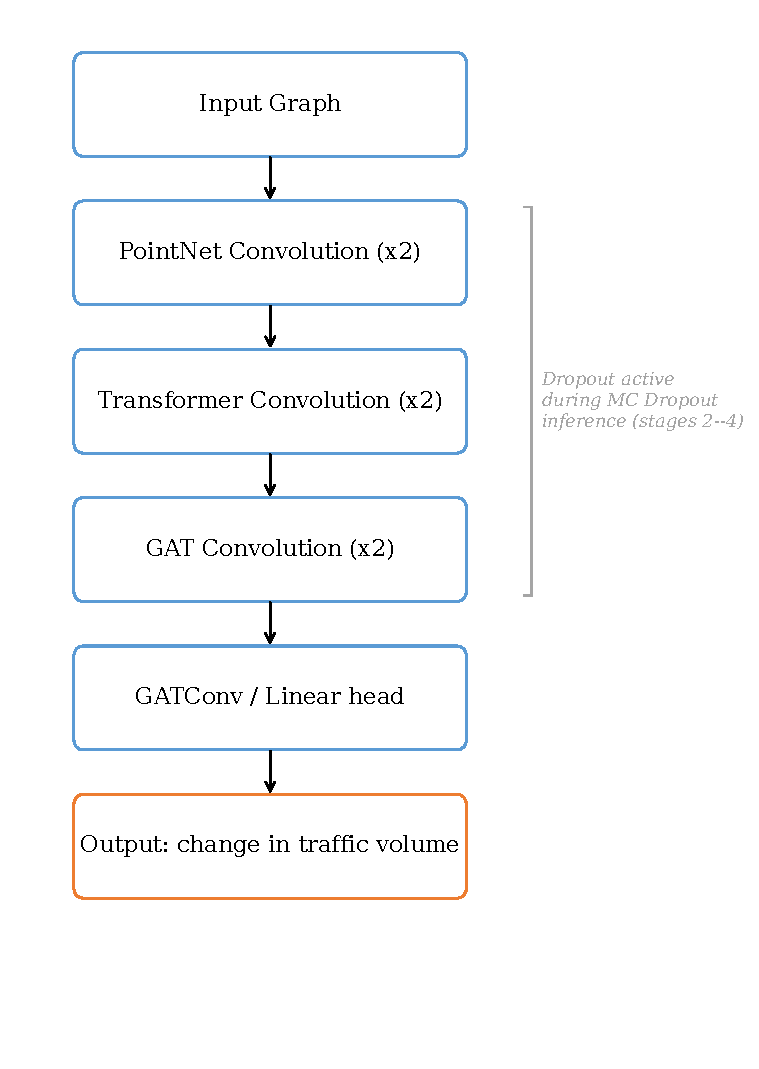
\includegraphics[height=0.6\textheight,keepaspectratio]{figures/new/fig29_pointnet_architecture.pdf}
 \caption[PointNetTransfGAT data flow]{Information flow through the PointNetTransfGAT architecture, top to bottom.\ The input graph is first encoded by two PointNetConv layers that extract local geometric features from each segment's start and end points.\ Two TransformerConv layers then capture longer-range relationships through self-attention across the network, two GATConv layers produce the final node embedding, and a final output layer (\texttt{GATConv(64$\to$1)} for T2--T8 and \texttt{Linear(64$\to$1)} for T1; see Table~\ref{tab:architecture}) produces the predicted change in traffic volume per node.\ Dropout, when enabled by the \texttt{use\_dropout} flag (T2, T5, T6, T7, T8), is applied within the PointNetConv MLPs and between the TransformerConv layers and remains active during MC Dropout inference for uncertainty estimation.}
 \label{fig:architecture}
\end{figure}

\section{Uncertainty Quantification Methods}\label{sec:uq_methods}

This thesis compares six UQ \emph{families} -- MC Dropout, seed-ensemble variance, multi-model ensembles, Deep Ensembles, heteroscedastic regression (Trial~9), and CQR (Trials~10--11) -- and three post-hoc calibration and deployment tools that compose on top of the families: split and adaptive conformal prediction, regression $\sigma$-scaling, and selective prediction.\ The mathematical formulations and references appear in Sections~\ref{sec:mc_dropout_bg}--\ref{sec:uq_metrics_bg} of Chapter~\ref{chapter:background}; this section specifies the procedural choices made in this thesis.

\paragraph{MC Dropout.}\ The trained model is evaluated $S = 30$ times with dropout active; per-node sample mean and standard deviation across passes form the prediction $\hat\mu$ and uncertainty $\hat\sigma$.\ A formal $S$-convergence study (Section~\ref{sec:s_conv_results}) confirms that $\rho$ has converged by $S = 30$, with the relative gain from $S = 30$ to $S = 50$ at $+1.03\%$.

\paragraph{Deep ensembles, single-architecture ensembles, and combined uncertainty.}\ Five PointNetTransfGAT models are trained from scratch with seeds $\{42, 137, 256, 389, 512\}$ (Trial~D); inference is deterministic and the inter-member spread is the uncertainty estimate.\ Two single-architecture variants are also evaluated: Experiment~A averages MC Dropout over five inference seeds of the same T8 model; Experiment~B is an $R^2$-weighted multi-model ensemble of T2/T5/T6/T7/T8.\ When MC Dropout and ensemble variance are both available, the two can be combined in quadrature, $\sigma_\text{combined} = \sqrt{\sigma_\text{MC}^2 + \sigma_\text{ens}^2}$.

\paragraph{Split conformal prediction (with an adaptive variant).}\ The 100-graph T8 test set is partitioned into 50 calibration and 50 evaluation graphs ($1{,}581{,}750$ nodes each); the nonconformity score is $|y - \hat y|$ (or $|y - \hat y|/\sigma$ for the adaptive variant), the quantile uses the standard $\lceil(n+1)(1-\alpha)\rceil/n$ correction (Section~\ref{sec:conformal_bg}), and intervals are constructed at $\{50, 70, 80, 90, 95\}\%$ coverage.

\paragraph{Post-hoc regression $\sigma$-scaling.}\ A single scalar $T > 0$ rescales the predictive standard deviation, $\sigma_\text{scaled} = T \cdot \sigma_\text{raw}$, with the point prediction $\hat\mu$ left unchanged.\ This is the regression analogue of, not an instance of, classification temperature scaling~\cite{guo2017calibration}: that procedure rescales softmax logits ($z \mapsto z/T$) to correct over-confident probabilities, whereas the regression variant rescales the predictive standard deviation ($\sigma \mapsto T\sigma$) to correct under-dispersed intervals -- same one-parameter, held-out, post-hoc structure operating on a different output channel.\ The rescaling is empirically warranted on the present continuous-valued $\Delta v$ task because the raw MC Dropout posterior is too concentrated~\cite{foong2019between}: at $T = 1$ the nominal $1\sigma$ Gaussian interval covers only $32.7\%$ of nodes against the $68.27\%$ Gaussian target (Section~\ref{sec:ts_results}), which is exactly the failure mode a single scalar $T > 1$ is designed to correct.\ Within this regression analogue, Kuleshov, Fenner and Ermon~\cite{kuleshov2018accurate} establish the regression-calibration framework (extending Platt-style classification calibration~\cite{guo2017calibration} to regression by recalibrating the predictive distribution on a held-out set), Laves~et~al.~\cite{laves2020wellcal,laves2019temperature} specialise it to MC Dropout regression as a single-scalar $\sigma$-scaling, and Levi~et~al.~\cite{levi2022evaluating} apply the same procedure to general regression heads.\ Under a Gaussian assumption on the recalibrated residuals, the maximum-likelihood estimator has the closed form $T^{\star 2}_\text{NLL} = N^{-1}\sum_i (y_i - \hat\mu_i)^2 / \hat\sigma_i^2$; on the present data this Gaussian-NLL estimator returns $T^\star_\text{NLL} \approx 6.35$ (Section~\ref{sec:ts_results}), reflecting the heavy-tailed component of the absolute-residual distribution rather than a calibrated bulk fit.\ We therefore fit $T$ by minimising the Kuleshov ECE~\cite{kuleshov2018accurate} on a $30\%$ random node-level subset of the test set (seed $42$, $949{,}050$ nodes) and evaluate on the remaining $70\%$.\ The ECE objective targets bulk-of-distribution coverage at $1\sigma$ rather than tail-weighted likelihood and is more robust to the heavy-tailed residuals observed here; the optimal value is $T^\star = 2.887$, which reduces ECE from $0.356$ to $0.034$ and brings $1\sigma$ coverage from $32.7\%$ to $68.0\%$ (Gaussian target $68.27\%$, Section~\ref{sec:ts_results}).

\paragraph{Selective prediction.}\ Predictions are sorted by $\sigma$ ascending and the most confident fraction $\tau$ is retained; MAE is reported on the retained subset.\ This characterises how much accuracy can be sharpened when an abstention budget is available.

\section{Evaluation Metrics}\label{sec:metrics}

The evaluation follows the metrics defined in Chapter~\ref{chapter:background}.\ Point-prediction quality is measured by $R^2$, MAE, and RMSE.\ Uncertainty ranking quality is measured by Spearman $\rho$ between $\sigma$ and $|y - \hat y|$.\ Calibration is reported via the Kuleshov ECE~\autocite{kuleshov2018accurate}, the conformal coverage probability $\mathrm{PICP}_{1-\alpha}$, and the empirical scaling factor
\begin{equation}\label{eq:kp}
 k_p = \mathrm{Quantile}\!\left(\left\{|y_i - \hat y_i|/(\sigma_i + \varepsilon)\right\}_{i=1}^{n};\ p\right),
\end{equation}
where $\varepsilon = 10^{-8}$ is a small numerical stability constant that avoids division by zero when $\sigma_i$ is close to zero.\ For a perfectly calibrated Gaussian, $k_{0.95} = 1.96$.\ Proper scoring rules, CRPS (Equation~\eqref{eq:crps_gaussian_bg}), the PIT, and the Winkler interval score, including the PIT KS statistic, are reported on the full $3{,}163{,}500$-node test set.\ Error detection is reported via AUROC at the top-$10\%$ and top-$20\%$ error thresholds, with AUPRC as the imbalance-aware companion.
